\documentclass{article}
\usepackage{graphicx}
\usepackage{float}
\usepackage{subfig}
\usepackage{fontspec}
\XeTeXlinebreaklocale "zh"
\XeTeXlinebreakskip = 0pt plus 1pt minus 0.1pt
\setmainfont{WenQuanYi Zen Hei}
\usepackage[top=1.2in,bottom=1.2in,left=1.2in,right=1in]{geometry}
\title{PIC}
\author{yan}
\date{\today}
\begin{document}
hello
world
你是个好人阿
          \begin{figure}
          \centering
            \subfloat[]{
	            \begin{minipage}[t]{0.5\linewidth}
	            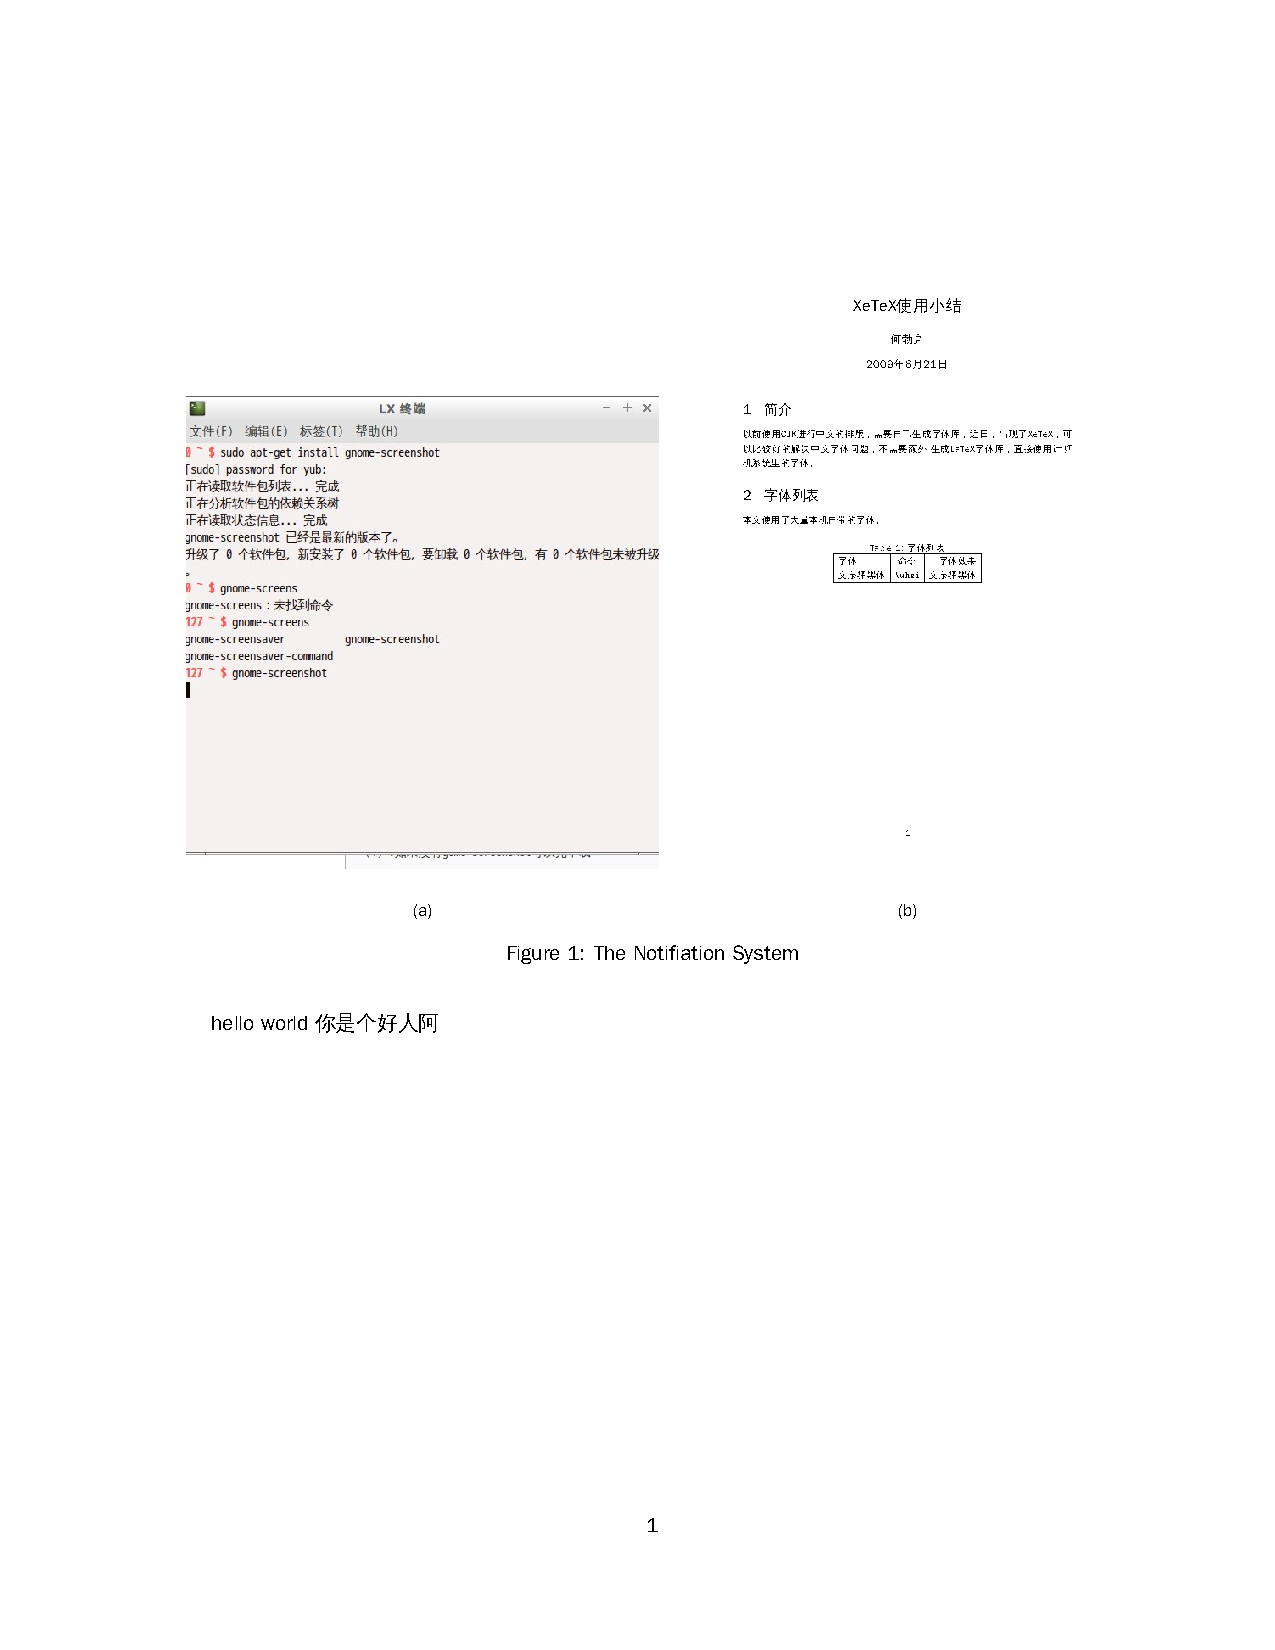
\includegraphics[width=\textwidth]{pic.jpg}
	            \centering
	            %\caption{(a)}
	            \label{fig:notification-sys:a}
	            \end{minipage}
	  }
            \subfloat[]{
	            \begin{minipage}[t]{0.5\linewidth}
	            \centering
	            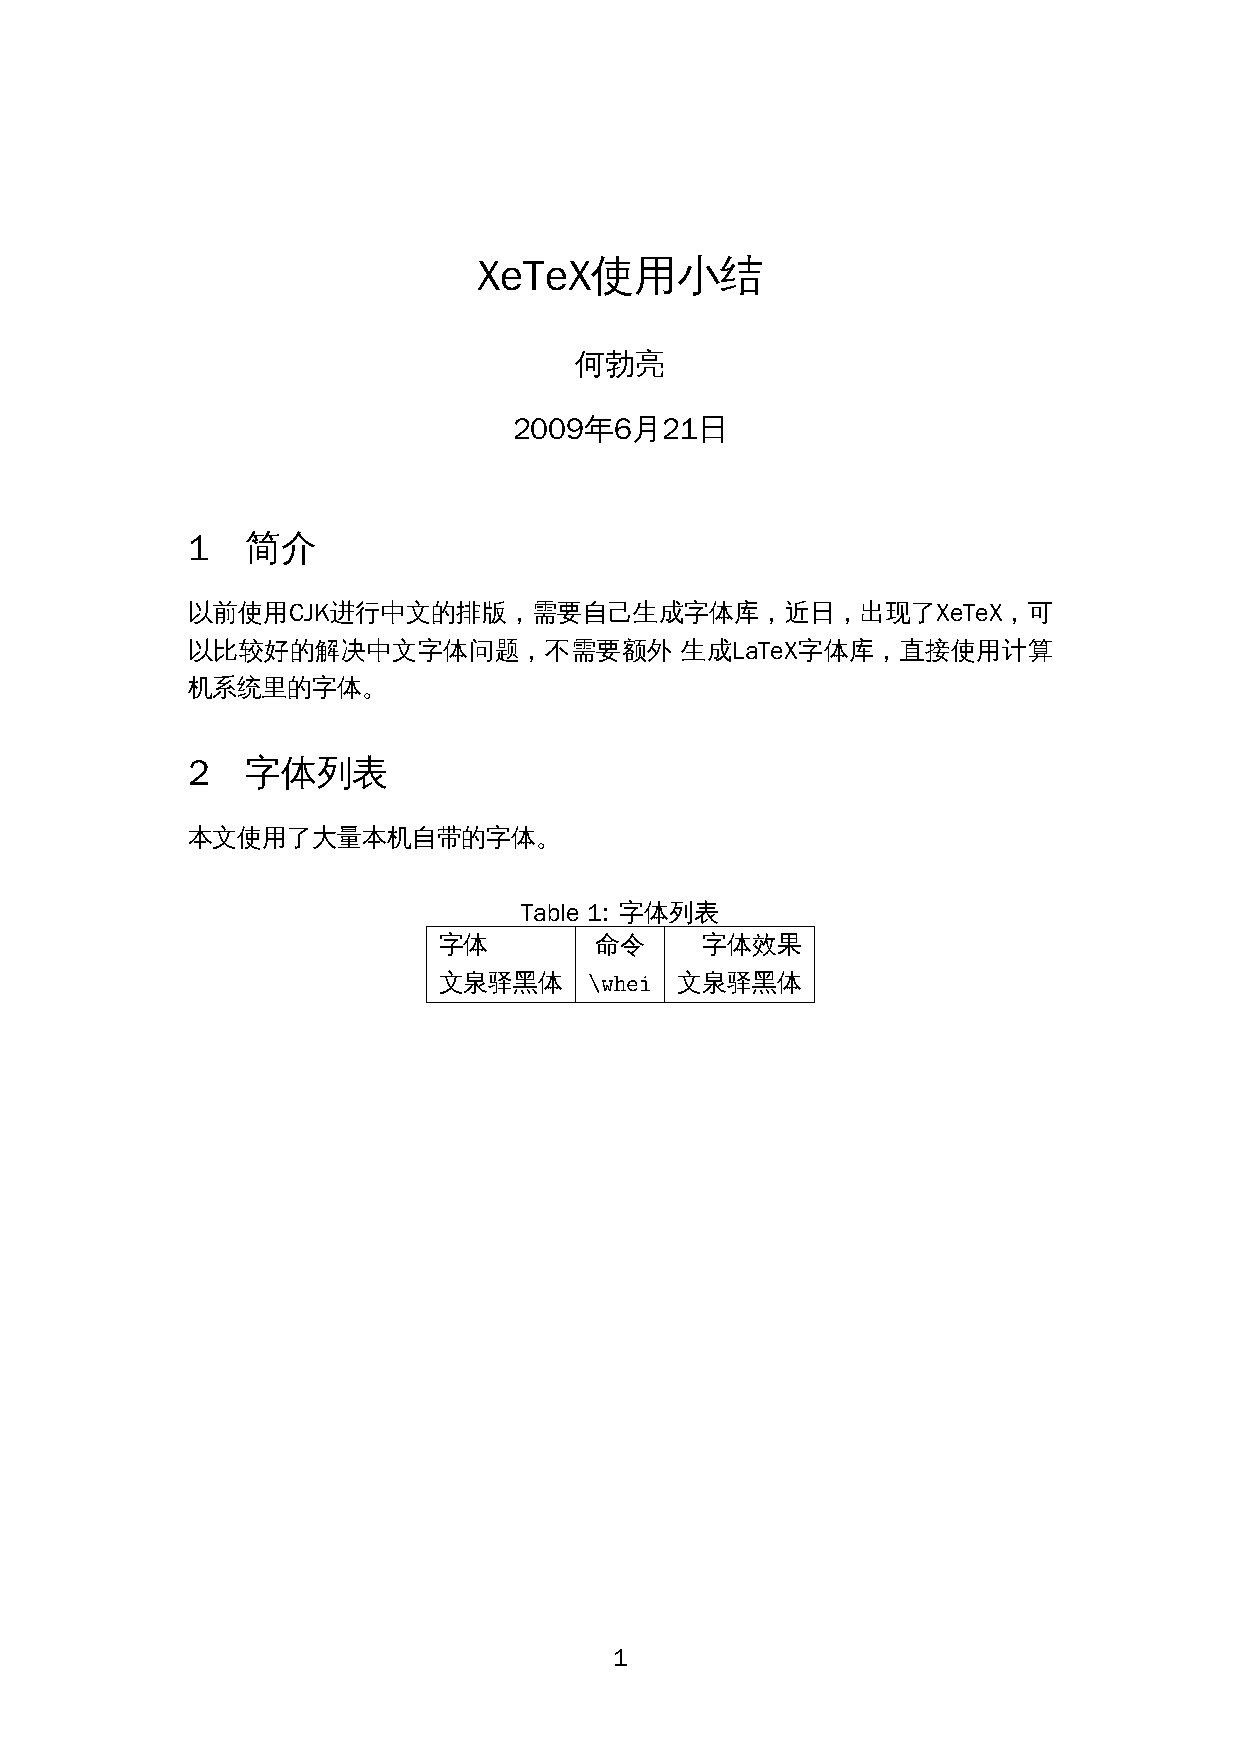
\includegraphics[width=\textwidth]{font}
	            %\caption{(b)}
	            \label{fig:notification-sys:b}
	            \end{minipage}
            }
          \caption{The Notifiation System}
          %\label{notification-sys}
          \end{figure}
\end{document}
